%%!TEX root = dissertation.tex

\chapter{Acknowledgments}

I am very fortunate to have had a deep support network throughout my degree at UBC and while writing this dissertation. First and foremost, my gratitude goes to Molly Babel---my advisor, mentor, collaborator, and friend. Molly supported me intellectually, creatively, and financially at all stages of my graduate career and dissertation writing adventure. I somehow stumbled into the perfect advising relationship, and I am so glad I did. I must also extend my gratitude to my committee members. Kathleen Currie Hall and Márton Sóskuthy both inspire me in different ways---encouraging me to think deeper, pursue open science practices, develop my technical expertise, and so much more. I know that my dissertation has less phonology in it than Kathleen may have hoped for, but I deeply appreciate her support for my research program, regardless of how closely it lined up with hers. This is the kind of supervisory committee I didn't know to hope for. 

I am also very grateful to my examining committee. Thank you for your enthusiasm and for joining me as I crossed the finish line. And to my external examiner---Matt Goldrick---your kind words and endorsement of my work means so much to me!

Other faculty in linguistics have inspired and pushed me to excel in many different ways. Carla Hudson Kam helped me through the qualifying papers process by pushing for a high standard of work while letting my not-quite-publishable study serve its purpose: learning. Henry Davis tried to get me to do a fieldwork dissertation, and while he was unsuccessful, it made me feel confident in what I did choose. 

In fall 2017, two seminars helped shape my research program in lasting ways. I am grateful to John Alderete and Henny Yeung at Simon Fraser University for their excellent seminar on the psycholinguistics of Chinese languages. In the same term, I also took an advanced phonetics seminar with Molly, and together, these seminars pushed me to think deeply about sound and psycholinguistics. Later in the program, I audited two quantitative methods courses with Márton Sóskuthy and Valter Ciocca, which helped me grow and gain confidence in my quantitative skills. My dissertation wouldn't be what it is without these amazing opportunities to learn.

This dissertation included creating a speech corpus from scratch. I would not have been able to do this without a fantastic team of research assistants. Ivan Fong and Nancy Yiu were active during all stages of the project---designing, recruiting, recording, and transcribing. They did it all. I am also grateful to everyone who contributed to the corpus, including Katherine Lee, Kristy Chan, Natália Oliveira Ferreira, Michelle To, Rachel Ching Fung Wong, Christina Sen, Ariana Zattera, and Rachel Soo. Creating the corpus would not have been possible without support from the UBC Public Scholars Initiative. I was able to submit and ultimately win an award, largely thanks to Serbulent Turan's tireless support of public scholars and Molly and Kathleen's encouragement to dream big. (And their support of my application, too!)

I would also like to thank everyone in the Speech-in-Context Lab for giving me feedback on earlier versions of my chapters, engaging with my ideas, and being the first group of people to use the corpus! I know that the lab will be the perfect home for the corpus over time. My dissertation also benefitted from feedback at various conferences---LREC, Interspeech, ASA meetings, and the Cantonese psycholinguistics workshop spearheaded by John Alderete.

Writing is hard and having a community helps. Thank you to Gloria Mellesmoen for our many writing sessions (particularly those where we didn't do any writing). It was the support I clearly needed, and it helped me keep a level head throughout the grad school roller coaster. While Gloria was the only person I managed regular writing time with, having an online writing community via 100 Days and Twitter was one of the more pleasant surprises of writing a dissertation in a pandemic. Knowing that we were all in it together made it so much better than it might have been.

Thank you to the grad students who were ahead of or overlapping with me in the linguistics program for showing me the ropes, answering my questions, going out for beers, and being all-around awesome people: Megan Keough, Oksana Tkachman, Emily Sadlier-Brown, Alexis Black, Natalie Weber, and many many others. And to my cohort---Gloria (again!), Roger Yu-Hsiang Lo, Wendy Amoako, Bruno Andreotti, and Daniel Reisinger. 

And lastly, to my friends and family. My parents have always supported me in following my linguistics career, and supporting me in this Ph.D. was no exception. Little did they know back when I started how this would launch my career. Thank you to my dad for all the (erudite) arguments over dinner and relentless word games. Thank you to my mom for always wanting to read my papers and for leading by example---we're both Dr. Johnson now! 

Thank you, in particular, to my amazing partner and husband, Brennan, for supporting me in so many ways. Whether it was driving up to Vancouver too many weekends out of the year in the early stages of my Ph.D. program or tearing me away from a midnight writing deadline in the middle of the pandemic for fancy takeout---that extra mile means the world to me. And to Pepper, dog and writing companion extraordinaire---she was impeccable in reminding me to take writing breaks, ideally outside. 15/10 work-from-home pal. 
\bigskip

\begin{figure*}[hb!]
    \begin{center}
    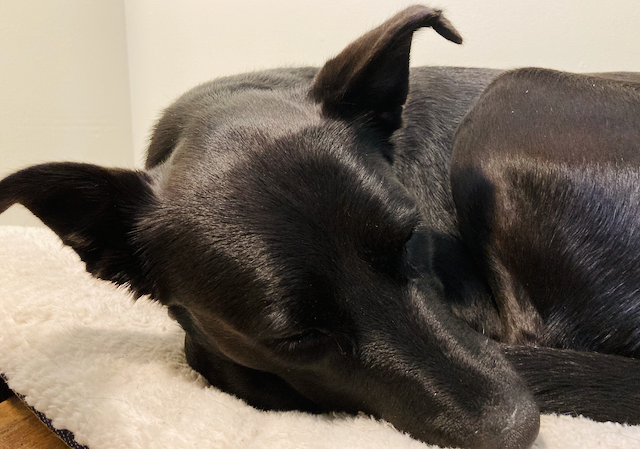
\includegraphics[width=3in]{figures/IMG_1228.png}     
    \end{center}
  \end{figure*}


\endinput % -------------------------------------------------------- %
